\documentclass[12pt]{article}
\usepackage{graphicx}
\usepackage{times}
\usepackage{cite}
\usepackage[utf8]{inputenc}
%this is a comment
\title{The Memo}
\author{Jesse Chick \& Benjamin Martin \& Keenan Johnson \& Nickoli Londura \& Jiaji Sun}




\begin{document}
\maketitle
\tableofcontents

\section{Contributors and ONIDs}
\begin{itemize}
	\item Jesse Chick $\sim$ chickj
	\item Benjamin Martin $\sim$ martinb3
	\item Keenan Johnson $\sim$ johnsoke
	\item Nickoli Londura $\sim$ londuran
	\item Jiaji Sun $\sim$ sunji
\end{itemize}

\section{Project Description}
\par
Learning to solve a Rubik’s cube blindfolded is a difficult task, especially if one is attempting to learn via random advice or unstructured memorization. Our users can improve their skills with our tool that is being developed by a team including an experienced blindfolded cuber. Our target audience for this web application will be those at a beginner or intermediate skill level learning to solve a 3x3 Rubik’s Cube blindfolded. There are a multitude of tutorials and resources for learning the methods of solving a cube blindfolded but very few tools exist that serve as teaching aids to practice and improve the newly learned skills. We aim to fill this gap in the community with an intuitive, easy-to-use web application.
\par 
Tutorials teaching the methods and information required to solve a cube blindfolded already exist. We are not an alternative to these tutorials. Instead, The Memo will serve as an intermediary aid to help practice and improve after the user has already learned the basics of blindfolded solving. The fact is, solving a cube blindfolded is quite different from solving normally. Memorization plays a key role in the task and the methods themselves are different. These new concepts can be difficult for those new to solving a cube blindfolded so we are striving to ease and aid the learning process.

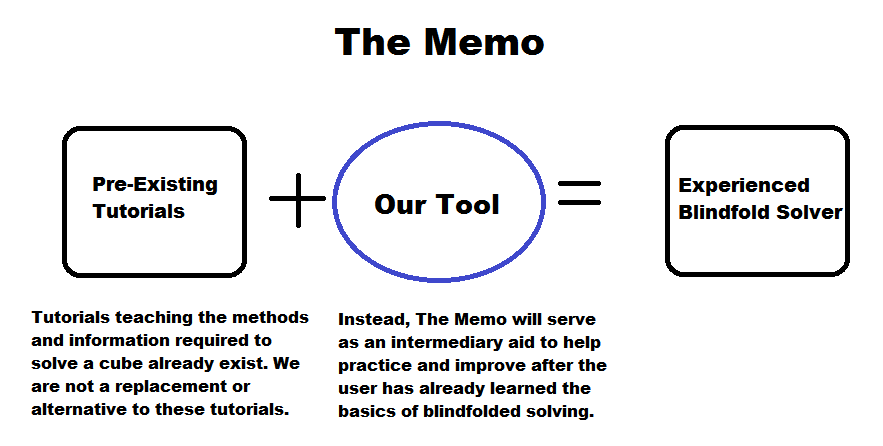
\includegraphics[width = \textwidth]{the_memo_diagram_shit.png}

\par
We will be creating a simple supplementary tool to aid those learning how to solve a 3x3 Rubik’s Cube blindfolded. Creating a web application is the simplest and most accessible form to create this tool and ensure that it’s intuitive to use. We’ll be using CSS and HTML for the organization and appearance of our content and then Javascript will be used to develop the functional aspects of our website and server side code. We don’t need any user data, so we don’t need any database plugins or code. We could expand on our project in this area later if we were to personalize the user experience.
\par
Our web application will have four main functions. It will…
\begin{itemize}
\item Show a visual representation of the letters on a virtual Rubik’s Cube.
\item Provide randomly generated scrambles along with corresponding letter solutions.
\item Create the letter strings that correspond to the memorization solution. 
\item Verify user input letter strings to ensure that their solution is correct. 
\end{itemize}
\par
As for non-functional features, we strive to create a tool that is visually pleasing with accurate colors that are clear and visible. We also aim to create a tool that is free of bugs that falls under the WYSIWYG mentality. The goal is to create an intuitive and easy-to-use web application. There will be basic instructions provided, but the user should have no issue or confusion when using our product. We will provide resources for tutorials on the subject as this tool is not a tutorial but rather an aid to practice and improve.

\par
As for possible additional features, the first idea is to store user data (success rates, memorization speed, other customizable features, etc.) so we can personalize the user experience. Another feature we could implement is one that generates easy to memorize words for given letter pairs. Example: given the letter pair CT would output an easy to memorize word such as ‘cat’.

\section{Use Cases}


\section{Planning}


\section{Meeting Report}


\section{Sources}


\end{document}
